\documentclass[10pt,twocolumn,letterpaper]{article}

\usepackage{cvpr}
\usepackage{times}
\usepackage{epsfig}
\usepackage{graphicx}
\usepackage{amsmath}
\usepackage{amssymb}


% Include other packages here, before hyperref.

% If you comment hyperref and then uncomment it, you should delete
% egpaper.aux before re-running latex.  (Or just hit 'q' on the first latex
% run, let it finish, and you should be clear).
\usepackage[breaklinks=true,bookmarks=false]{hyperref}

\cvprfinalcopy % *** Uncomment this line for the final submission

\def\cvprPaperID{****} % *** Enter the CVPR Paper ID here
\def\httilde{\mbox{\tt\raisebox{-.5ex}{\symbol{126}}}}

% Pages are numbered in submission mode, and unnumbered in camera-ready
%\ifcvprfinal\pagestyle{empty}\fi
\setcounter{page}{1}
\begin{document}

%%%%%%%%% TITLE
% \title{Random variables in Communication network}
\begin{titlepage}
\centering

{\Huge \bfseries Probability and Random Processes\\}
\vspace{3cm}
{\huge Probability and Random Processes in Communication network\\}
\vspace{4cm}
{\huge Group Number:5\\}
\vspace{4cm}
{\large 
Shantanu Chauhan: 2020112002\\
Pranav Manu: 2020112019\\
Varshita Kolipaka: 2020113007\\
Srujana Vanka: 2020102005\\}

\vspace{2cm}
Github Repo: \href{https://github.com/hohilwik/PRP-project}{Click Here}
\end{titlepage}




%\thispagestyle{empty}

%%%%%%%%% ABSTRACT
% \begin{abstract}
%   The ABSTRACT is to be in fully-justified italicized text, at the top
%   of the left-hand column, below the author and affiliation
%   information. Use the word ``Abstract'' as the title, in 12-point
\begin{onecolumn}

{\Huge \centering Introduction\\}
\vspace{0.5cm}
\large
The report focuses on the applications of probability of Random Process on communication networks. It will discuss the implementation of probability on computer networks, analyzes the performance of a computer network, simulates a system, and looks into some design issues that affect performance.The report will also elaborate on dependence of Random variable which is widely used in the field of Communication to make effective and efficient communication and compression models. Probability can be used to make inferences about the transmitted message based on the received message. This is even more helpful when communication takes place over a noisy channel. It will also cover compression methods, specifically Arithmetic Code, its applications, benefits, the general methodology and predictions using a probabilistic model. Lastly, an example of forward error correction, Reed Solomon Code, is discussed.
\end{onecolumn}
\newpage
\twocolumn
%--------------------------------------------------------------------------
\section{Introduction [5]}

Computer communication networks are ubiquitous and have many configurations including local 
area networks (LANs), wireless networks, satellite networks, and Internet. If we consider single link, series link and parallel link networks given in figure 1, the probability that a packet is damaged on a computer link is p. We consider each of the network models and analyze performance of the network based on the values of p. Specifically, we are interested in the probability of packet losses in the network and the expected number of packet transmissions for a large number of packets. 

We begin with an email that is broken into K packets and then transmitted over a computer link. The probability of losing a packet is p. If a packet is damaged, it is re-transmitted. Here we also discuss the Bernoulli and geometric distributions, and their means and variances. In addition, we address the probability that a packet is transmitted successfully in at most two tries, and move on to N tries, and then address the design factors that influence the choice of N. Then we move on to the entire e-mail and the average number of packets sent for a successful e-mail over serial and parallel links and consider the reliability of both, 

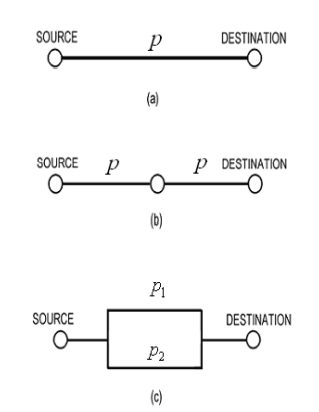
\includegraphics[width=\linewidth]{plots/fig1.PNG}
\caption{Figure 1. Basic network structures; (a) single link, (b) series link, (c) parallel link}

\section*{Single Link Network{\small[1][3][5]}}

Consider an e-mail being transmitted across a single network link. The e-mail is broken up into K packets, each of which is transmitted individually across the link. The probability that a transmission fails is p, and in the case of a failed transmission, the packet is re-transmitted. The probability p may depend on many factors, including the type of link such as wireless, wired, or optical, the number of people sharing the link, the physical distance traveled across the link, environmental conditions, and the error correction techniques. If there are many users sharing a network, then several users might compete for network resources and initial transmission attempts might fail due to packet collisions. 

Here we notice that the random variable indicating the outcome of a single transmission is either a success or a failure and follows a Bernoulli distribution. 

The probability that the packet is successfully sent after $n$ transmission is given by 
$$p^{n-1}(1-p)$$
(the transmission must fail $n-1$ times, each with probability $p$, and then succeed on the $n^{th}$ try).

Here we define the random variable Y to be the number of transmissions for a successful transmission of a packet. We note that Y is a geometrically distributed random variable and plot its probability mass function and its cumulative distribution function.

The average number of transmissions $E(Y$ for a successful transmission of a packet is
$$ E(Y) = \sum_{i=0}^{\infty} ip^{i-1}(1-p)= 1/(1-p) $$

A quick check of the boundary conditions shows that if $p=0$ (all transmissions succeed), then the expected number of transmissions is 1, while if $p=1$ (all transmissions fail), infinitely many transmissions are required. We show a plot of the expected number of transmissions vs p.

Ideally, packets are transmitted in as few transmissions as possible. Suppose for instance that we would like the packet to travel across the link after no more than two tries. The probability of that occurring is

$$ q_{1,2} = (1-p)+p(1-p)= 1-p^2 $$

(the sum of probabilities that the packet will arrive after exactly one or exactly two attempts or 1 minus the probability of two failures in two tries). For instance, if p=0 and all attempts succeed, then only one transmission is required. However, if p=1, the probability is zero. We show a plot of the probability of success in at most two tries vs p.

Generally speaking, the probability that a packet is successfully transmitted across one network link in at most N tries is

$$ q_{1,N} = \sum_{i=1}^{N} p^{i-1}(1-p) = 1-p^N $$

Therefore, for values of $p$ less than one (a non-zero probability of transmission success), the probability that the packet will be eventually transmitted successfully approaches 1 as N increases without bound. The next figure shows a plot of the probability success vs $p$. At this point, we discuss the effects of $p$ and $N$ on the network performance.

If a packet is transmitted N times without success, the sender should be notified that a failure has occurred and to try again later. The choice of $N$ depends on the number of users on the network and traffic patterns observed by the network managers, transmission medium, environmental conditions, and network delay. For instance, if a user is working late at night when there is virtually no competing network traffic, and repeated attempts at sending a packet fail, then the error is probably due to a network failure instead of competition. On the other hand, if multiple users are attempting to send information across a network at the same time, more transmission attempts should be made before deciding that the problem is due to a network failure.

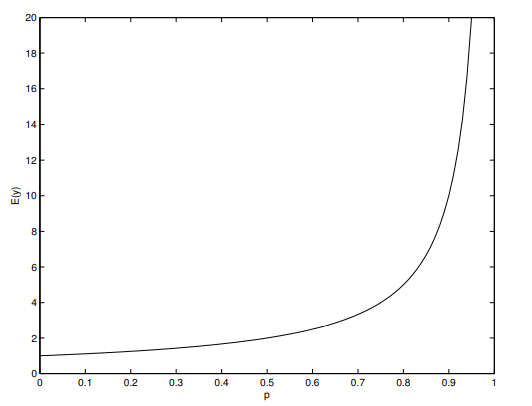
\includegraphics[width=\linewidth]{plots/fig2.PNG}
\caption{Figure 2: The average number of transmissions required to send one packet across a single link}

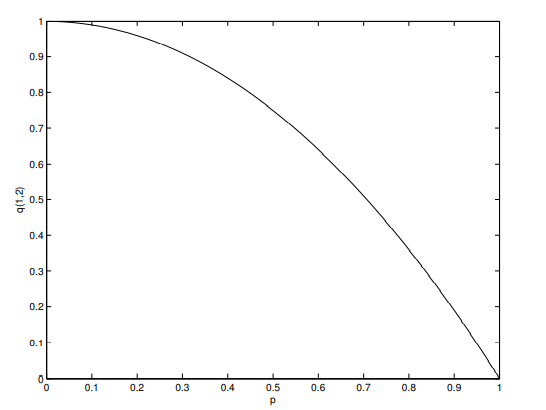
\includegraphics[width=\linewidth]{plots/fig3.PNG}
\caption{Figure 3: The probability that a single packet will be sent without error across a single link}

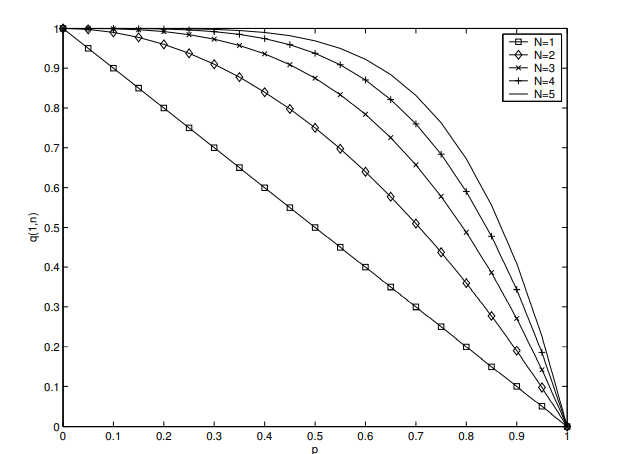
\includegraphics[width=\linewidth]{plots/fig4.PNG}
\caption{Figure 4: The probability that a single packet will be sent without error in at most N tries, for N=1 to N=5}



\section*{Single Link: Multiple Packets{\small[3][4][5]}}

An email will be partitioned into several packets before being transmitted over the network. Suppose there are $K$ packets, each of which is transmitted separately. Depending on the values of $p$ and $K$ packets, it may be very unlikely for the entire message to transmit on the first attempt. All packet transmissions must succeed, making this probability

$$ Q_K = (1-p)^K $$

This is plotted for several values of K.

Suppose that packets are sent over the network in succession, and if any packet transmission fails, the failed packet is re-transmitted until success occurs. Packets successfully transmitted before a later packet fails are not resent. We define the random variable $Z$ to be the average number of transmissions required for a successful transmission of the entire email. 

$E(Z)$ can be computed easily since the success or failure of any packet transmissions is independent from the other $K-1$ transmissions, and we found earlier that a single packet takes on an average, 1/(1-p) transmissions to succeed, so we expect that the complete set of K packets will be transmitted in K/(1=p) attempts. 

We can use a simulation to verify experimentally that K/(1-p) is the correct probability expression. The MATLAB program in $packet_transmission.m$ runs N simulations for set values of p and K and counts the number of transmissions required, then averages over the N experiments. Sample runs were performed with the following parameter sets:

\begin{itemize}
    \item N=1000, K=5, p=0.5
    \item N=1000, K=11, p=0.47
\end{itemize}
 
 The mean transmission counts for these two experiments were, respectively, 9.972 and 20.817. Theoretical values derived from our previous discussion are 10.0 and 20.8, which agree with the results of our simulation. A histogram of the transmission count for the 1000 simulations with p=0.5 is plotted. This plot demonstrates how the values are concentrated around the theoretical value of 10.
 
 As we have observed, this type of network raises some serious concerns about system reliability. For any file partition consisting of a large number of packets, many transmissions are expected before the file is sent in its entirety. This number grows rapidly with increasing probability of packet damage on a link. When considering the two remaining network structures, we will return to this issue as a basis for comparison. 

At this point, we assume K, the length of an email message, is a random variable with an exponential distribution. 

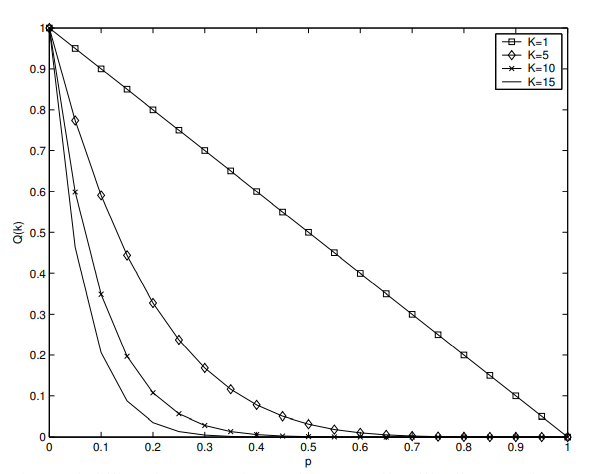
\includegraphics[width=\linewidth]{plots/fig5.PNG}
\caption{Figure 5: The probability that K packets of an email will all transmit across one link successfully in the first attempt for K=1,5,10,15}

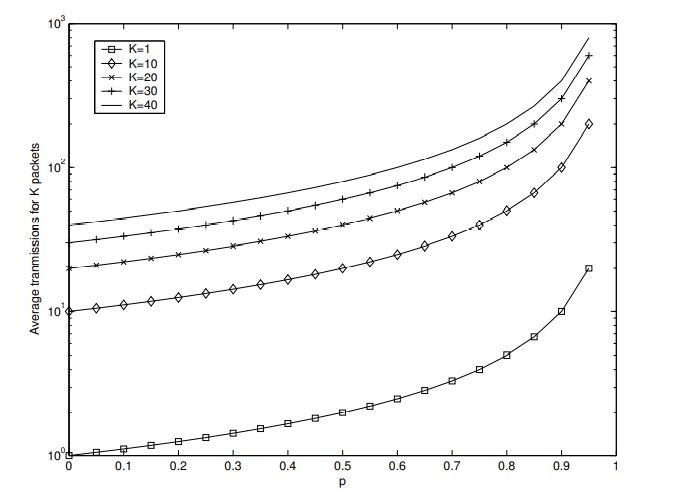
\includegraphics[width=\linewidth]{plots/fig6.PNG}
\caption{Figure 6: The expected number of transmissions required to send K packets across one network link without error for K=1,10,20,30,40}

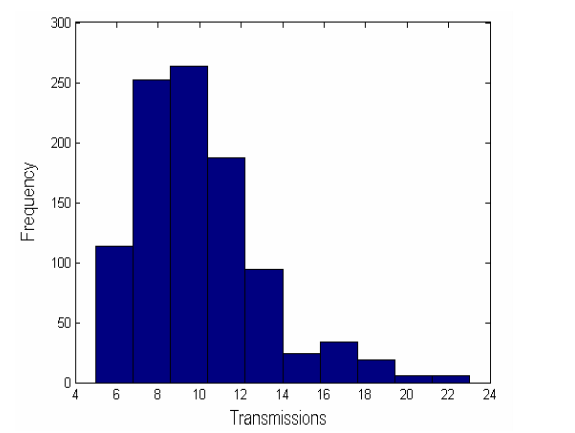
\includegraphics[width=\linewidth]{plots/fig7.PNG}
\caption{Figure 7: Histogram of transmissions required to send 5 packets across a single link, whose probability of failure is 0.5, for 1000 simulations}


\section*{Series Two-Link Network\small{[1][2][5]}}

Suppose that each packet in the K-packet email must be transmitted across two network links connected in series. The probability of losing a packet on any one link is still p. During the transmission process, if a packet is damaged on any one of the two links, it must be re-transmitted across the first link again.

The probability that a packet is transmitted successfully across both links in the network is $(1-p)^2$ because a successful transmission with probability $(1-p)$ must succeed in two consecutive, independent trials. We plot this probability and compare it to the probability that a transmission across a single network link succeeds. 

An email composed of K packets is much less likely to transmit successfully on the first try. In such a case, all K packets must transmit successfully across two links, or a total of 2K successful transmissions. This occurs with probability $(1-p)^{2K}$ and is plotted vs p for several values of K.

Now let Z be the random variable representing the number of times a packet is transmitted over the first link until it is received successfully. If a packet transmission fails, we must send the packet across both links again. Let $q_{2,k}$ be the probability that the packet is transmitted successfully in exactly k tries, Then $q_{2,k}$ can be expressed as the following recursion:

$$ q_{2,1} = (1-p)^2 $$
and $ q_{2,k} = (1-\sum_{j=1}^{k-1} q_{2,j})(1-p)^2 $

In order for the attempt to succeed on the $k^{th}$ try, all previous attempts must have failed. The probability that the attempt succeeded for some $j<k$ is $\sum_{j=1}^{k-1} q_{2,j}$, so the probability that it failed is $1- \sum_{j=1}^{k-1} q_{2,j}$. Finally, the $k^{th}$ attempt must succeed, so we have the $(1-p)^2$ term at the end. We derive the non-recursive form as:

$$ q_{2,k} = (1-\sum_{j=1}^{k-1} q_{2,j})(1-p)^2 $$
$$ q_{2,k} = (1-p)^2 - (1-p)^2 \sum_{j=1}^{k-1} q_{2,j} $$
$$ q_{2,k} = q_{2,k-1} - (1-p)^2 q_{2,k-1} $$
$$ q_{2,k} = p_{k-1} (1-(1-p)^2) $$
$$ q_{2,k} = q_{2,2} (1-(1-p)^2)^{k-1} $$
$$ q_{2,k} = (1-p)^2 (1-(1-p)^2)^{k-1} $$

Then the average number of transmissions required to send a single packet across is given by 

$$ E(Z) = \sum_{k=1}^{\infty} k(1-p)^2 (1-(1-p)^2)^{k-1} = 1/(1-p)^2 $$

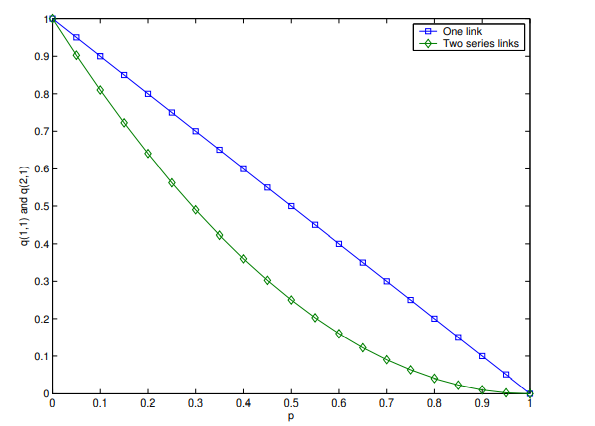
\includegraphics[width=\linewidth]{plots/fig8.PNG}
\caption{Figure 8: The probability that one packet will transmit across a network without error on the first attempt for a one-link and series two-link connection}

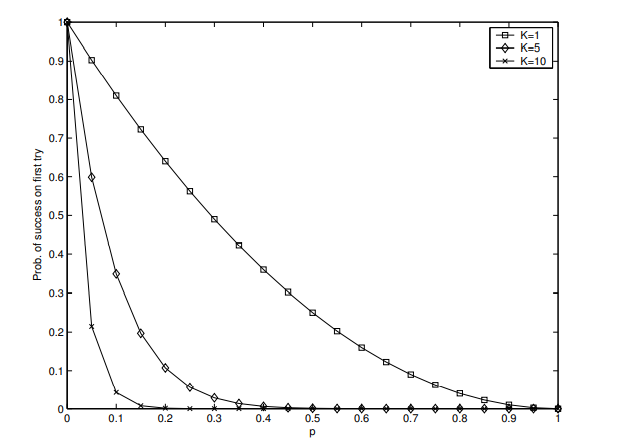
\includegraphics[width=\linewidth]{plots/fig9.PNG}
\caption{Figure 9: the probability that all K packets of an email will transmit across the series network on the first attempt for K=1,5,10,15,20}

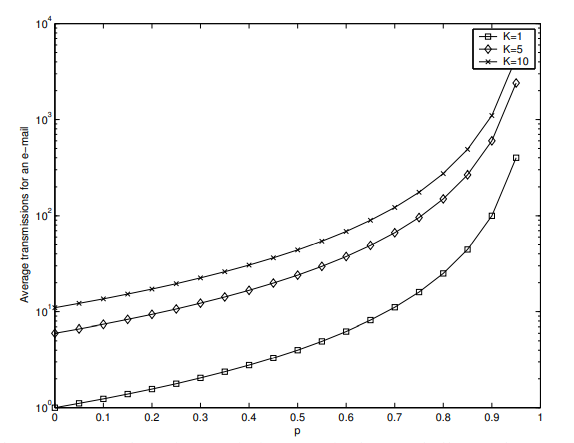
\includegraphics[width=\linewidth]{plots/fig10.PNG}
\caption{Figure 10: The average number of transmissions required to send all K packets across the series network without error (log scale) for K=1,6,11,16,21}


However, our email has K separate packets, each of which takes an average of $1/(1-p)^2$ transmissions, Therefore, the total number of expected packet transmissions for the email is $K/(1-p)^2$. We plot this function vs p for several values of K. Simulations were performed to verify this expression and the results agreed strongly with the analytical prediction. 

If we already assume that a packet is transmitted successfully over the first link, it is much easier to compute the probability of a successful transmission across the network. The probabilities of successful transmission across either link are independent; then the probability that the packet is transmitted without error over the second link, given that it was transmitted correctly over the first link, is (1-p).

The series-link connection exhibits a poorer overall performance than the single-link network. The simple explanation for this is that a greater number of transmissions must take place, increasing the chances that failures will occur.

Let us define the random variable W to be the number of transmissions across both links for successful transmission. We can compute E(W) by noting that:

$$ q_{2,2} = (1-p)^2 $$
$$ q_{2,3} = p(1-p)^2 $$
$$ q_{2,4} = p q_{2,3} + (1-p) p q_{2,2} $$
$$ ... $$
$$ q_{2,k} = p q_{2,k-1} + p (1-p) q_{2,k-2} $$

where $q_{2,k}$ is the probability of success in k transmission on both links and p is the probability of failure on a link

$$ E(W) = \sum_{k=2}^{\infty} k q_{2,k} = \frac{2-p}{(1-p)^2} $$

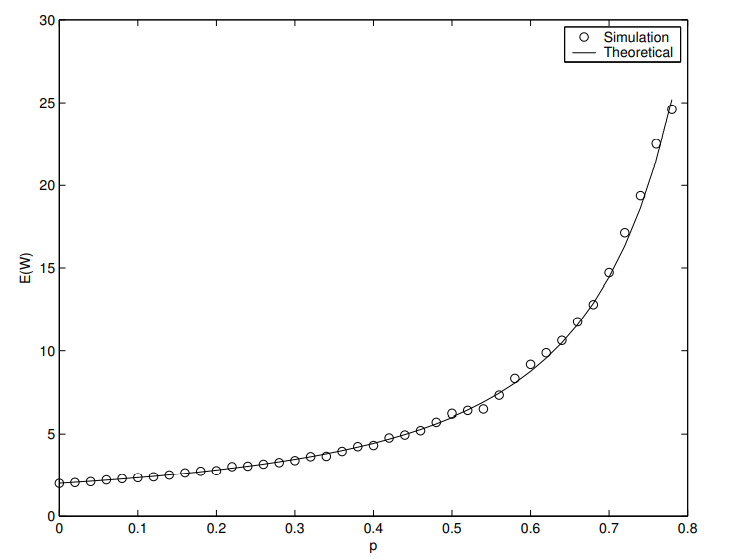
\includegraphics[width=\linewidth]{plots/fig11.PNG}
\caption{Figure 11: the average number of transmissions across two links vs p}


\section*{Series Multiple-Link Network{\small[5]}}

Now suppose that we have a network of k links, all in series, and that we would like to transmit a single packet across all the links. As before, damage occurs with probability p, and once a packet is damaged, it is lost along the entire network and must be re-transmitted from the first node. The number of packets $N_k$ that we should expect to send, extending our derivation from before, is:

$$ N_k = \frac{1-(1-p)^k}{p (1-p)^k} $$

A quick check of the boundary conditions shows that $N_k \to \infty$ as $p$ nears one, and $N_k \to k$ as $p$ approaches zero, which is what we expected.

\section*{Parallel Two-Link Network{\small[1][2][5]}}

Suppose that our network consists of two links connecting a pair of common nodes (a parallel network). The probability that a packet is damaged during a transmission across the two links is $p_a$ and $p_b$, respectively. The packet travels across both links to arrive at the destination. The packet will reach its destination through both links with a probability of $(1-p_a)(1-p_b)$, since the transmissions must succeed on both links simultaneously. If $p_a=p_b$, then the probability reduced to $(1-p_a)^2=(1-p_b)^2$.

The packet transmission is considered successful if the packet travels across either parallel link without getting damaged. This occurs with probability $(1-p_a p_b)$ because the only chance that the transmission is unsuccessful is if failure occurs in both links. If $p_a=p_b$, the packet will arrive with probability $(1-p_a^2$. We plot the previous functions for this parallel network. We can argue from the results considered in this, that of the three network types considered, the parallel network provides the highest probability of transmissions success on the first try. The intuitive reason for this is that there are the most independent paths to the destination in this type of network design, which increases the chances that the packet will travel successfully across $one$ of them.

Since the e transmission successes across the two links are statistically independent events, we can summarize with the following observations: 
\begin{itemize}
    \item Given that the packet is correctly received across the first link, the probability that the packet is transmitted correctly on the second link is $(1-p_b)$
    \item Given that the packet is damaged along the first link, the probability that it is transmitted correctly on the second link is still $(1-p_b)$
\end{itemize}

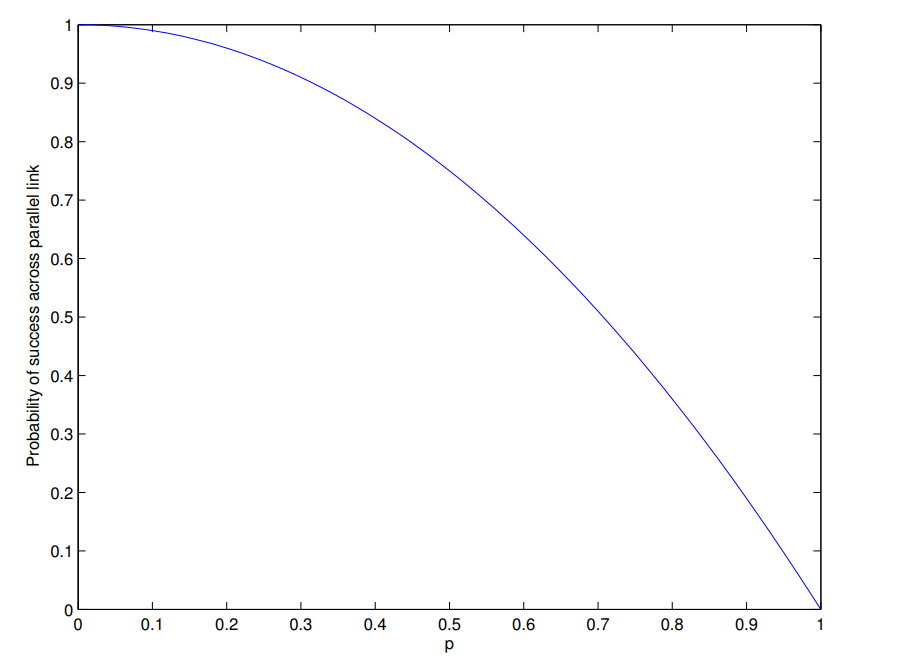
\includegraphics[width=\linewidth]{plots/fig12.PNG}
\caption{Figure 12: The probability that a single packet travels without error through both links of a parallel network on the first attempt}

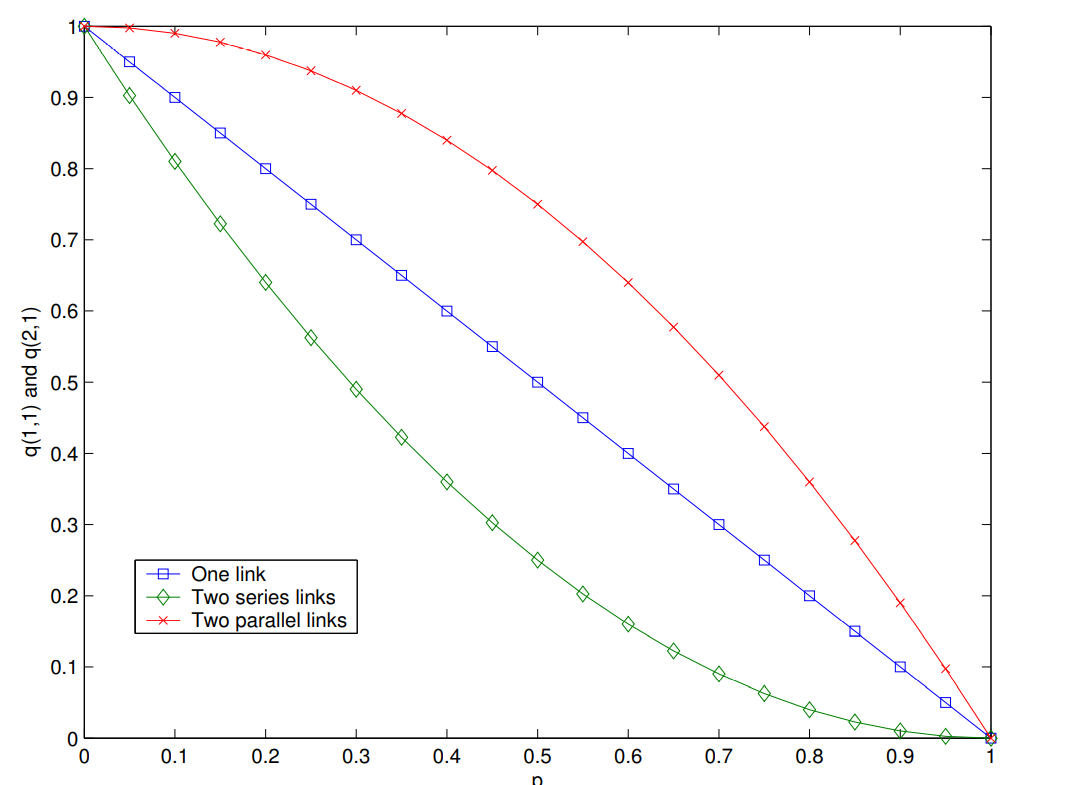
\includegraphics[width=\linewidth]{plots/fig13.PNG}
\caption{Figure 13: the probability that one packet will be transmitted across a network without error on the first attempt for one-link, series two-link, and parallel two-link connections}


The parallel-link network exhibits the best behavior of the three structures we have examined. Because more links connect a common pair of routers, there is a higher chance that a transmission will succeed because only one of the links needs to pass the packet through undamaged. The situation is analogous to the two-input digital OR and AND logic gates; assuming that all input combinations are equally likely, there is a higher chance that the output of the OR gate will be logical HIGH because only one of its inputs needs to be HIGH, while both of the inputs to the AND gate need to be HIGH for the same output condition. In this case, the series network acts like an AND gate and the parallel network acts like an OR gate.

%--------------------------------------------------------------------------
\section{Dependent Random variables in Communication{\small[9]}}

We use Random vectors with independent components can be used to represent information in Communication network. However, in real world, it is not so as each component may be correlated to the other in some way and if we know this correlation we can perform better compression.To understand the correlation, we must know the models of dependence. Another application of dependent random variable is when a sequence of bits is transmitted through a noisy channel, then the sequence received at receiver, in the form of a random vector, depends on the transmitted random vector. If they were independent, then we could never be able to decode the received back to the original message with low probability.
%-------------------------------------------------------------------------
\subsection{Forward and inverse probability}
Probability calculations fall into two categories: \textit{forward probability} and \textit{inverse probability}.
\textbf{Forward probability} involves some generative model that describes a process that results in some data, the task then becomes to compute the probability distribution or expectation of some quantity that depends on the data. Entropy calculation falls into this category.\\
\textbf{Inverse probability} problems also involve some generative model of a process (In this discussion, this process is communication), but here instead of calculating the probability distribution of some quantity as a result of the process, we calculate the probability of one or more unobserved variables in the process, given the observed variables. This concept will be used ahead in the modelling of a decoder to estimate the transmitted sequence, given a received sequence in communication. This involves the use of Bayes' Theorem, and can be used in predictions. It can also be used in data compression.
\subsubsection{Inferences in Probability}
Inference in communication involves deciphering the message transmitted through a noisy channel upon receiving it at the receivers end. Inferences can be correctly made in communication networks using the Bayes' theorem.

\subsection{Types of Entropy}

The following Entropy will be used ahead. Entropy can be said as the expected information content carried by a Random variable.\\
\textbf{Entropy}:
\begin{eqnarray*}
H(X)&=&\sum_{x\in Supp(P_{X})}{P_{X}(x).log\frac{1}{P_{X}(x)}}
\end{eqnarray*}
\textbf{Joint Entropy}:
\begin{eqnarray*}
H(X,Y)&=&\sum_{x,y\in Supp(P_{X,Y})}{P_{X,Y}(x,y).log\frac{1}{P_{X,Y}(x,y)}}
\end{eqnarray*}
Here the entropy represents the expected information carried by X and Y simultaneously.\\
\textbf{Conditional Entropy}:
\begin{eqnarray*}
H(X \vert Y)&=&\sum_{y\in Supp(P_{Y})}{P_{Y}(y).H(X \vert Y=y)}\\
H(X|Y=y)&=&\sum_{x\in Supp(P_{X|Y})}{P_{X|Y}(x|y).H(x|y)}
\end{eqnarray*}
This represents the expected information carried by X, given that we know the information in Y.
It can also be described as the uncertainty that remains in X after we know Y, as information is the increases as uncertainty increases. We can see that the conditional entropy depends on the conditional probability of X given Y.
For independent X and Y:
\begin{eqnarray*}
H(X|Y)=H(X)
\end{eqnarray*}
This can be explained by the fact that since they are independent, knowing Y we still cannot say anything about X.\\
\textbf{Information Content and chain rule}:
Information content of X is represented as:
\begin{eqnarray*}
    \frac{1}{p_X(X=x_i)}
\end{eqnarray*}
And chain rules of probability states that for two random variables:
\begin{eqnarray*}
    p(x,y)=p(x).p(y|x)
\end{eqnarray*}
Using this in the expression for entropy, we can derive the chain rule for Entropy:
\begin{eqnarray*}
    H(X,Y)=H(X)+H(Y|X)=H(Y)+H(X|Y)
\end{eqnarray*}
\textbf{Mutual induction}:
\begin{eqnarray*}
I(X;Y)\equiv H(X)-H(X|Y)=H(Y)-H(Y|X) 
\end{eqnarray*}
This is used to represent the reduction in information content after we have received Y, or vice versa. This concept is used to define the \textbf{channel capacity} or the maximum amount of information that can be sent through a channel. This can also express the average information content expressed by one about the other. 

\subsection{Gibbs Inequality}
Also known as relative entropy or Kullback-Leibler divergence between two probability distribution $P(x)$ and $Q(x)$ defined over the same alphabet $A_X$, it is a very important concept in information theory. It can loosely be used to define the "distance" between two probability distributions. However it is not strictly distance. It is not symmetric, that is, relative entropy between P and Q is not the same as the relative entropy between Q and P.
\begin{eqnarray*}
    D(P||Q)=\sum_{x}P(x).log\frac{P(x)}{Q(x)}
\end{eqnarray*}


\section{Communication over a noisy Channel{\small[9]}}
Channels, or the medium through which information is transmitted, are usually noisy. The need arises develop methods for error-free communication.For this purpose, we will elaborate on noisy error channel and channel coding. Channel coding is used to make the noisy channel behave close to a noiseless channel. The Channel Code is made such that noisy signal received can be decoded. As we have stated before, the measure of the information  transmitted can be expressed by the mutual information between the transmitted and received signal.

%-------------------------------------------------------------------------
\subsection{Noisy Channels}

Conditional probability between the transmitted signal and the received signal can be used to characterize the noisy channel.\\
\textbf{Discrete Noiseless Channel(Q):}
It is characterized by an input alphabet $A_X$ an output alphabet $A_Y$ (Alphabet is the set of values that the message can be mapped to) , and a set of conditional probability distributions $P(y |x)$, one for each $x\in A_X$ .
\begin{eqnarray*}
    Q_{j|i}=P(y=b_j|x=a_i)
\end{eqnarray*}
We can make this into a matrix such that each column is a probability vector, and then obtain the $P_Y$ probability vector by multiplying Q matrix with $P_X$ probability vector.
% \begin{verbatim}
% \thispagestyle{empty}
% \end{verbatim}
Some models of noisy channel are:
\textbf{Binary Symmetric Channel:} $A_X$={0,1}. $A_Y$={0,1}
\begin{eqnarray*}
P(y=0|x=0)=1-p;\ P(y=1|x=0)=p\\
P(y= 0|x= 1)=p;\ P(y= 1|x=1) = 1-p\\
\end{eqnarray*}
Here p is said to be the probability of the transmitted bit to be flipped.\\
\textbf{Binary Erasure Channel:} $A_X$={0,1}. $A_Y={0,\epsilon,1}$
\begin{eqnarray*}
P(y=0|x=0)=1-p;\ P(y=1|x=0)=0\\
P(y= \epsilon|x= 1)=p;\ P(y= \epsilon|x=1)= p\\
P(y=1|x=0)=0;\ P(y=1|x=1)=1-p
\end{eqnarray*}
Here p is said to be the probability of the transmitted bit getting erased. $\epsilon$ represent the erasure of the bit. The bit is not flipped here, but erased with some probability.
The probability of getting erased or flipped in the above noisy channels is conditionally dependent on the transmitted bit.

%-------------------------------------------------------------------------
\subsection{Estimating the input given the output}
To estimate the transmitted symbol x from the received signal y, we can use the \textbf{Bayes' theorem} given y:
\begin{eqnarray*}
P(x|y)&=&\frac{P(y|x).P(x)}{P(y)}\\
&=&\frac{P(y|x).P(x)}{\sum_{x_i\in X}P(y|x_i)P(x_i)}
\end{eqnarray*}
A decent estimate here is: $\underset{x}{argmax}(P(x|y))$

\subsection{Information conveyed by a Channel}
    To measure the amount of information the output conveys about particular input X, we use mutual Information:
    \begin{eqnarray*}
        I(X;Y)\equiv H(X)-H(Y|X)
    \end{eqnarray*}
    Note that:$I(X;Y)\leq min(H(Y),H(X))$. Intuitively it means that no more than the conveyed information can be received.
    \textbf{Maximising mutual information}\\
    Maximising mutual information conveyed by the channel would mean to maximise the amount of information transferred in communication. We define the channel capacity of a channel Q to be the maximum mutual information over $P_X$
    \begin{eqnarray*}
        C(Q)=\underset{P_X}{max}I(X;Y)
    \end{eqnarray*}
    We have control over $P_X$ and can maximising it by optimising the input coding. $P_X$ at channel capacity is called \textit{optimal input distribution}. The rate can be increased only up to the channel capacity if we want to have arbitrarily small probability of error. This is the converse of the \textbf{Shannon's Channel Coding theorem.}

\subsection{Optimal Decoder for noisy channel coding}
Since the transmitted sequence or codeword might have some error due to it being transmitted  though a noisy channel. As a result, the received codeword is not the same as the transmitted one. Therefore, a need arises to infer the transmitted message from the received codeword, to enable communication. This is done by the use of a decoder.
For a channel, an optimal decoder is one which minimises the probability of error. It decodes an output y as the input x that has maximum posterior probability P(x|y)
\begin{eqnarray*}
    P(x|y)&=&\frac{P(y|x).P(x)}{\sum_{x_i\in X}P(y|x_i)P(x_i)}\\
    \hat{x}_{optimal}&=&argmax P(x|y)
\end{eqnarray*}
If the prior distribution on x is uniform, then the optimal decoder is called \textit{maximum likelihood decoder} i.e., the estimation is such that the output is such that P(y|x) has the maximum likelihood.

\subsection{Gaussian Random variable to model Noise}
Noise can also be modelled using Gaussian random variable. Noise can be defined as the sum of infinitely many independent random variable, as there may be several disturbances in the channel. According to \textit{Central Limit theorem}, sum of infinitely many independent random variable results is a Gaussian random variable. The resultant sum can be said as the random variable representing the noise in the channel.
%-------------------------------------------------------------------------
%% S's


% Include other packages here, before hyperref.

% If you comment hyperref and then uncomment it, you should delete
% egpaper.aux before re-running latex.  (Or just hit 'q' on the first latex
% run, let it finish, and you should be clear).





% Pages are numbered in submission mode, and unnumbered in camera-ready
% \ifcvprfinal\pagestyle{empty}\fi

% %%%%%%%%% TITLE
% \title{\LaTeX\ Author Guidelines for CVPR Proceedings}


% For a paper whose authors are all at the same institution,
% omit the following lines up until the closing ``}''.
% Additional authors and addresses can be added with ``\and'',
% just like the second author.
% To save space, use either the email address or home page, not both
% \and
% Second Author\\
% Institution2\\
% First line of institution2 address\\
% {\tt\small secondauthor@i2.org}
% }

% \maketitle
%\thispagestyle{empty}

% %%%%%%%%% ABSTRACT
% \begin{abstract}
%   The ABSTRACT is to be in fully-justified italicized text, at the top
%   of the left-hand column, below the author and affiliation
%   information. Use the word ``Abstract'' as the title, in 12-point
%   Times, boldface type, centered relative to the column, initially
%   capitalized. The abstract is to be in 10-point, single-spaced type.
%   Leave two blank lines after the Abstract, then begin the main text.
%   Look at previous CVPR abstracts to get a feel for style and length.
% \end{abstract}


%%%%%%%%% BODY TEXT
\section{Entropy rates of a Stochastic Process{\small[7]}}


A stochastic process, also called a random process, is a set of random variables that model a non deterministic system.  Many time-varying signals are random in nature, such as noises, image and audio: usually unknown to the distant receiver. Random process (or stochastic process) presents the mathematical model of these random signals. If the random variables are dependent or in particular, if the random variables form a stationary process, we will show, just as in the i.i.d.case, that the entropy
\begin{math}H (X 1 , X 2 , \dots , X n )\end{math} grows (asymptotically) linearly with n at a rate \begin{math}H ( X )\end{math}, which we will call the entropy rate of the process.

An indexed sequence of random variables is called a stochastic process
\begin{math}
{X_i}\end{math}. 
There can be arbitrary dependencies among random variables in general. The joint probability mass functions characterise the process.\\
\begin{math}
Pr\{(X_1 , X_2 , \dots , X_n )=(x_1 , x_2 , \dots, x_n )\} = p(x_1 , x_2 , \dots , x_n ), (x_1 , x_2 , \dots ,x_n ) \in X_n \quad for \quad n = 1, 2, \dots
\end{math} \\
\\
\textbf{Definition} A stochastic process is said to be stationary if the joint
distribution of any subset of the sequence of random variables is invariant
with respect to shifts in the time index; that is,\\
\begin{math}
{
\begin{mathbf}
Pr\{X_1 = x_1 , . . . , X_n = x_n \}
= Pr\{X_1+l = x_1 , . . . , X_n+l = x_n \}
\end{mathbf}
}\end{math}
for every n and every shift l and $\forall x_1 , x_2 , \dots , x_n \in X$ .
\subsection{Markov chains}
An example of a stochastic process with dependency is one in which each random variable is conditionally independent of all the other previous random variables.

Markov is the name for such a process.\\
\textbf{Definition} A discrete stochastic process\begin{math}
X_1 , X_2 , \dots 
\end{math} is said to be a
Markov chain if for n = 1, 2, \dots , \\
\\
$
\begin{mathbf}
Pr(X_{n+1} = x_{n+1} |X_n = x_n , X_{n-1} = x_{n-1} , . . . , X_1 = x_1 )
= Pr (X_{n+1} = x_{n+1} |X_n = x_n )
\end{mathbf}$\\

\begin{math}
\quad \forall \quad x_1 , x_2 , . . . , x_n , x_{n+1} \in X .
\end{math}\\ 
\\
In this case, the joint probability mass function of the random variables
can be written as\\
\\ \begin{math}
p(x_1 , x_2 , \dots, x_n ) = p(x_1 )p(x_2 |x_1 )p(x_3 |x_2 ) · · · p(x_n |x_{n-1} ).
\end{math}\\
\\ It is assumed that the Markov chains are time invariant unless otherwise
stated. \\
\\ \textbf{Definition} The Markov chain is said to be time invariant if the conditional probability \begin{math} p(x_n+1 |x_n )\end{math} does not depend on n; that is, for n = 1, 2, \dots , 
\begin{eqnarray*}
\\ Pr\{X_{n+1} = b|X_n = a\} = Pr\{X_2 = b|X_1 = a\} 
\end{eqnarray*} \begin{math} \forall \quad  a, b\in X .\end{math} \\
\\
\textbf{State and Transition matrix:} \\ If \begin{math} {X_i} \end{math} is a Markov chain, \begin{math} X_n \end{math} is called the state at time n. A time-invariant Markov chain is characterized by its initial state and a probability transition matrix, given by
\begin{math}
 P = [P_{ij} ], \quad for \quad i, j \in {1, 2, \dots , m}, 
\end{math}
\\ where \begin{math} P_ij = Pr\{X_{n+1} = j |X_n = i\}. \end{math} \\
\\
If it is possible to go with positive probability from any state of the
Markov chain to any other state in a finite number of steps, the Markov
chain is said to be \textbf{irreducible}. \\If the largest common factor of the lengths
of different paths from a state to itself is 1, the Markov chain is said to
\textbf{aperiodic}.\\
\\ 
\textbf{Example: }Consider a two-state Markov chain with a probability transition matrix given by: 
 \begin{eqnarray*}
\begin{bmatrix}
{1 - \alpha} & \alpha \\
\beta & 1 - \beta
\end{bmatrix}
\end{eqnarray*}
\\
Let's say the stationary distribution is represented as a vector \begin{math}
 \mu \end{math} with the stationary probabilities of states 1 and 2 as its components. Then, by solving the equation \begin{math}
  \mu P = \mu \end{math} or, more simply, by balancing probabilities, the stationary probability can be obtained. 
  \begin{equation*}
      \mu P = \mu \implies \mu P = \mu I \implies \mu(P - I) = 0 
  \end{equation*}
  \\The net probability flow across any cut set in the state transition graph is zero for the stationary distribution. \\ As \begin{math}
   \mu \end{math} is a probability distribution it follows that \begin{math} \mu_1 + \mu_2 = 1. \end{math} \\ Solving for \begin{math} \mu\end{math}, using the above and the following equation, \quad
\begin{math}
      \mu_1\alpha = \mu_2\beta.
\end{math} The stationary distribution is given by:
\begin{equation*}
    \mu_1 = \frac{\beta}{\alpha + \beta}, \: \mu_2 = \frac{\alpha}{\alpha + \beta}
\end{equation*} 
The resulting process will be stationary if the Markov chain has an initial state drawn according to the stationary distribution. The entropy of the state \begin{math} X_n
\end{math} is: \\
\begin{equation*}
    H(X_n) = H( \frac{\beta}{\alpha + \beta}, \frac{\alpha}{\alpha + \beta} ).
\end{equation*}\\
\subsection{Entropy Rate}
Since a stochastic process defined by a Markov chain that is irreducible, aperiodic and positive recurrent has a stationary distribution, the entropy rate is independent of the initial distribution. is the asymptotic distribution of the chain.\\
\\ \textbf{Definition: }The entropy of a stochastic process \begin{math} {X i } \end{math} is defined by
\begin{equation*}
    H(X) = \lim_{n \to \infty} {\frac{1}{n}}H(X_1,H_2, \dots H_3)
\end{equation*} when the limit exists.\\
\\We can also define a related quantity for entropy rate:
\begin{equation*}
    H'( X ) = \lim_{n \to \infty} H (X_n |X_{n-1} , X_{n-2} , . . . , X_1 )
\end{equation*} when the limit exists.\\
\\\begin{math}
      H(X) 
\end{math} and \begin{math}
      H'(X)
\end{math} are two different notions of entropy rate. The first is the entropy of the n random variables per symbol, and the second is the conditional entropy of the last random variable given the past. \\ We now show that both limits exist and are identical for stationary processes.\\
\\ \textbf{Entropy of a stationary Markov Chain:}\\
For a stationary Markov chain, the entropy rate is given by
\begin{equation*}
    H ( X ) = H'( X ) = \lim H (X_n |X_{n-1} , . . . , X_1 ) 
\end{equation*}
\begin{equation}
= \lim H (X_n |X_{n-1} )
= H (X_2 |X_1 )
\end{equation}\\
\textbf{Theorem: }Let \begin{math}
      \{X_i\}
\end{math} be a stationary Markov chain with stationary distribution µ and transition matrix P . \\Let \begin{math}
      X_1  \char`\~ \mu
\end{math} Then the entropy rate is
\begin{equation*}
    H(X) = -\sum_{ij}\mu_i P_{ij} \log{P_{ij}}
\end{equation*}
\textbf{Proof}
\begin{equation*}
    H ( X ) = H (X_2 |X_1 ) 
\end{equation*}
\begin{equation*}
   = \sum_i \mu_i(\sum_j -P_{ij}logP_{ij})
\end{equation*}
%-------------------------------------------------------------------------
\subsection{Functions of Markov chains}
Let $ X 1 , X 2 , \dots , X n , \dots $ be a stationary Markov chain, and let $ Y_i = \varphi (X_i)$ be a process each term of which is a function of the corresponding state in the Markov chain. To compute $H ( Y )$, we might compute $H (Y_n |Y_{n-1} , . . . , Y_1 )$ for each n and find the limit.
Upper and lower bounds converging to the limit from above and below might be advantageous computationally. When the difference between the upper and lower bounds is small, we can stop the computation and get a solid estimate of the limit.\\ We know that  \begin{math}  H (Y_n |Y_{n-1} , . . . , Y_2 , Y_1 )  \end{math} converges to \begin{math} H(Y) \end{math} i.e, \begin{math} H (Y_n |Y_{n-1} , . . . , Y_2 , Y_1 )  \leq H(Y) \end{math}\\
\\The lemma shows that the interval between the upper and the lower bounds decreases in length.\\
\\ \textbf{Lemma}\\
\begin{equation*}
    H (Y_n |Y_{n-1} , . . . , Y_1 ) - H (Y_n |Y_{n-1} , . . . , Y_1 , X_1 ) \to 0.
\end{equation*}
\textbf{Proof}
\\The LHS can also be written as:
\begin{equation*}
     H (Y_n |Y_{n-1} , . . . , Y_1 ) - H (Y_n |Y_{n-1} , . . . , Y_1 , X_1 )
\end{equation*}
\begin{equation*}
    = I (X_1 ; Y_n |Y_{n-1}, . . . , Y_1 )
\end{equation*}
This mutual information is always less than or equal to \begin{math}
H(X_1) \end{math} i.e, 
\begin{equation*}
    I (X_1 ; Y_1 ,Y_2 , . . . , Y_n  ) \leq H(X_1)
\end{equation*} 
As n tends to infinity, \begin{math}\lim I (X_1 ; Y_1 ,Y_2 , . . . , Y_n ) \end{math}
exists.\\ From the chain rule, 
\begin{equation*}
    H (X) \geq \lim_{n \to \infty} I (X_1 ; Y_1 , Y_2 , . . . , Y_n )
\end{equation*}
\begin{equation*}
    = \lim_{n \to \infty} \sum_{i=1}^{n} I (X_1 ; Y_i |Y_{i-1} , . . . , Y_1 )
\end{equation*}
\begin{equation*}
    = \sum_{i=1}^{\infty} I (X_1 ; Y_i |Y_{i-1} , . . . , Y_1 )
\end{equation*}
As n tends to infinity, this sum of infinite terms is finite and the terms are non-negative, the terms must tend to 0; which proves the lemma, that is,
\begin{equation*}
    \lim I (X_1 ; Y_n |Y_{n-1} , . . . , Y_1 ) = 0
\end{equation*}
From this lemma, we have the following theorem:\\
\\ \textbf{Theorem:}\\
If \begin{math} X_1 , X_2 , . . . , X_n \end{math} form a stationary Markov chain, and
\begin{math} Y_i = \varphi(X_i ) \end{math}, then 
\begin{equation*}
    H (Y_n |Y_{n-1} , . . . , Y_1 , X_1 ) \leq H ( Y ) \leq H (Y_n |Y_{n-1} , . . . , Y_1 )
\end{equation*}
and
\begin{equation*}
   \lim H (Y_n |Y_{n-1} , . . . , Y_1 , X_1 ) = H ( Y ) 
\end{equation*}
similarly, 
\begin{equation*}
    \lim H (Y_n |Y_{n-1} , . . . , Y_1 ) = H(Y)
\end{equation*}
\begin{math}
\end{math}
\subsection{Use of stochastic processes in communication{\small[8]}}

We are all aware that all communication systems both generate and are affected by noise. Since to implement any circuit or device whether in Analog or Digital domain, we need it’s Mathematical Model, without which we cannot implement anything. It provides us with a method or metric to use in real-world circumstances. The same may be said for noise. Random process (also known as stochastic process) is an area of mathematics that can develop or apply mathematical models for noise in communication systems.

Because of its time fluctuating character, noise is modelled as a random variable, which is then modelled as a random process. Because it closely reflects the probability distribution of the noise that occurs in communication systems, Gaussian Noise is the most famous model for noise in communication systems today.

So in this way the random process or also known as Stochastic Process is useful in Communication Systems.


%-----------------------------------------------------------------------------
\section{Compression Methods}
Here 2 compression methods have been discussed:
1. \textbf{Arithmetic coding} A method that is based on the principle that a compression of data from a source entails probabilistic modelling of that source. 
2. \textbf{Lempel–Ziv coding}: A Single compression algorithm that works decently for most kinds of sources. This compression is widely used and often effective.

%-------------------------------------------------------------------------
\subsection{Arithmetic codes{\small[9]}}

These rectify problems in the problems that occur in the Huffman codes.  In an arithmetic code, the probabilistic modelling is
separated from the encoding operation. The probabilistic model of the source behaves as a predictor here. 
Now, we know that each symbol is produced by the source and the probabilistic model provides a predictive distribution over the possible values of the next symbol

We choose a source alphabet: $A_x = \{a_1, \dots a_i\}$. Let the last symbol, $a_i$ indicate the end of transmission. 
We assume that the source produces an arbitrary and a not necessarily i.i.d sequence, something of this sort: $x_1\dots x_m\dots x_i$
We assign a predictive probability distribution over $a_i$ (over the current sequence) 
\begin{equation}
   P(x_n = a_i \vert x_1,\dots, x_{n-1}) 
\end{equation}
We consider an example below.\\
\emph{Example: compressing the tosses of a bent coin}\\
Let us simulate an experiment where we toss a bent coin a number of times, and name the outcomes as a and b.
There is an additional possibility wherein we encounter an EOF symbol, analogous to the one in the previous case.
This is not a biased coin, so we don't expect the outcomes of $a$ and $b$ to be equal.

From this simulation, let string $s$ be a source string. \\
\begin{center}
    $s = bbba$\\
\end{center}


\subsubsection{Encoding}
After passing the string for computation character by character. We calculate the probability of obtaining a either $a$ or $b$ or EOF given the context.
Context is basically the sequence so far. Here "*" indicates the EOF
\\
xx
\begin{table}[htbp]
    \begin{tabular}{|l|l|l|l| }
    \hline
    Context & P(A$\vert$Context)     & P(B$\vert$Context)    & P(C$\vert$Context)     \\
    \hline
    -       & P(a)=0.425       & P(b)=0.425      & P(*)=0.15        \\
    \hline
    b       & P(a$\vert$ b)=0.28    & P(b $\vert$ b)=0.57   & P(* $\vert$ b)=0.15    \\
    \hline
    bb      & P(a$\vert$bb)=0.21   & P(b $\vert$ bb)=0.64  & P(* $\vert$ bb)=0.15   \\
    \hline
    bbb     & P(a$\vert$bbb)=0.17  & P(b $\vert$ bbb)=0.68 & P(* $\vert$ bbb)=0.15  \\
    \hline
    bbba    & P(a$\vert$bbba)=0.28 & P(* $\vert$ bbb)=0.57 & P(*$\vert$bbba)=0.15 \\
    \hline
    \end{tabular}
    \end{table}

\includegraphics[scale=0.4]{encoding_arithmetic.png}
The above graphic from the Information Theory Learning and Algorithms Book. 
It demonstrates the encoding process for the string $s$
\\ 
\subsubsection{Analysis of the Process}

When the first symbol 'b' is observed, the encoder is aware that the string must begin with the
string 01, 10, 11, but without a surity of which exactly. Nothing is written yet, and the next character is examined
. In our case it is 'b'. Now this is an interval 'bb' lies completely interval '1'. Now the encoder can finally write the first bit: '1'. 
The consequent 'b' narrows the interval range further. However this isn't enough for us to ascertain whether this belongs in the '10' interval. 
After the 'a' is read, we can transmit more bits. The interval 'bbba' lies completely the interval '1001'. 
Hence, '001' is added to '1' previously written by the encoder. 

When the EOF arrives, we terminate the encoding process by a procedure which we shall abstract away here. 
Finally, upon magnifying the interval 'bbba' we note that an interval '100111101' is completely contained by 'bbba'. Hence, now we can append '11101'.
\subsubsection{Overhead to Terminate}
We note that the overhead bits required to terminate a message is never more than 2 bits (subject to the message length)\\
Let the underlying probabilistic model be $\mathcal{H}$. $h(x \vert \mathcal{H}) = log[1/P(x | \mathcal{H})].$
\\
\\
\\
\\
\\
\\
\\
\\
\\
\\
\subsubsection{Decoding}

In the encoding process we have transmitted the string '100111101' and one-by-one the characters are passed to the decoder. 
Using a procedure similar to that used in the encoding, the probabilities of obtaining a,b, and EOF. 
Because the interval ‘10' fits entirely within interval ‘b', it is evident that the original string must have began with a ‘b' once the first two bits ‘10' have been inspected.
\\
The decoder may then utilize the model to determine the bounds of the intervals ‘ba', ‘bb', and ‘b' by computing $P(a \vert b)$, $P(b \vert b)$, and $P(* \vert b)$. Continuing, we decode the second b when we reach ‘1001', the third b when we reach ‘100111', and so on, until we achieve the unambiguous identification of ‘bbba' after reading the entire binary string.
When we encounter the EOF, the decoder knows that it must stop decoding. 


\subsubsection{Predictions by a probabilistic model}
One can produce intervals defined by a simple bayesian probabilistic model. The interval size is proportional to the probability of the occurance of the strings
In such a model we can assign a constant ratio to the frequencey of occurance of each character. 
\begin{equation} 
    P_L(a \vert x_1, . . . , x_{n-1}) = \frac{F_a + 1}{F_a + F_b + 2}
\end{equation}
\\
Here $F_a(x_1, \dots, x_{n-1})$ is the frequency of the occurance of a so far. $F_b$ is the number of b's.\\

\subsection{Forward Error Correction (Reed-Solomon Code){\small[10][11]}}
An example of a forward error correction code is Reed-Solomon code. The working consists of oversampling a polynomial that is derived from the data
. The polynomial is evaluated at several points. Sampling the polynomial more than required makes it over-determined. This way, upon receiving the too many points, even if a few errors occur in transmission, the errors can be known. Polynomial Algorithms can be used to obtain the original word.
Reed-Solomon codes are examples of block codes. This implies that a fixed block of the input data is processed into another packaged block of output data. 

\subsubsection{Concept (Basic)}

The essential concept underlying a Reed-Solomon code is that the data is viewed as a polynomial first. The code is based on an algebraic theory that says that any $k$ distinct points define a polynomial with a degree of at most $k-1$.
Over a finite field, the sender chooses a degree $k-1$ polynomial to represent the  $k$ data points. The polynomial is subsequently "encoded" at various places by its evaluation, and these values are what is really delivered.

\subsubsection{Error Correcting Mechanism}
For practical Reed–Solomon coding applications, it is common to use a finite field $F$ with $2^m$ components. In this situation, each symbol may be represented by a $m$-bit value. The transmitter sends the data points in encoded blocks, with each encoded block containing $n=2^m-1$ symbols.
As a result, each block of an $8$-bit Reed–Solomon code includes $n=2^8-1=255$ symbols. (This is a very popular value due to the prominence of byte-oriented computer systems.) The amount of data symbols in the block ($k$, with $k \leq n$) is a design parameter.

\subsubsection{Optimal Application Areas}
Because of the qualities stated above, Reed–Solomon codes are well-suited to circumstances where errors occur in bursts. Reason: the code doesn't care how many bits are incorrect in a symbol; if several bits are incorrect in a symbol, it counts as a single error.

\newpage
\onecolumn

\begin{thebibliography}{}
\bibitem{1}Roy D. Yates and David J. Goodman, Probability and Stochastic Processes: A Friendly Introduction for Electrical and Computer Engineers, 2005
\bibitem{2}T.T. Soong, Fundamentals of Probability and Statistics For Engineers, 2004
\bibitem{3}Rodger E. Ziemer, Elements of Engineering Probability and Statistics, 1997
\bibitem{4}Athanasios Papoulis and S. Unnikrishan Pillai,Probability, Random Variables and Stochastic Processes, 2002
\bibitem{5}William Stallings, Data and Computer Communications, 2000
\bibitem{6}Elements in Information Theory-Thomas M. Cover, Joy A.Thomas
\bibitem{7}Basics of Applied Stochastic Processes- Serfozo
\bibitem{8}Probability Theory and Stochastic Processes with Applications, Oliver Knill
\bibitem{9}Information Theory Learning and Algorithms by David J.C. MacKay
\bibitem{10}Reed \& Solomon (1960)
\bibitem{11}D. Gorenstein and N. Zierler, "A class of cyclic linear error-correcting codes in p\^m symbols", J. SIAM, vol. 9, pp. 207-214, June 1961 Error Correcting Codes by W\_Wesley\_Peterson, 1961
\bibitem{12}Error Correcting Codes by W\_Wesley\_Peterson, second edition, 1972
\bibitem{13}Yasuo Sugiyama, Masao Kasahara, Shigeichi Hirasawa, and Toshihiko Namekawa. A method for solving key equation for decoding Goppa codes. Information and Control, 27:87–99, 1975.
\bibitem{14}Immink, K. A. S. (1994), "Reed–Solomon Codes and the Compact Disc", in Wicker, Stephen B.; Bhargava, Vijay K. (eds.), Reed–Solomon Codes and Their Applications, IEEE Press, ISBN 978-0-7803-1025-4
\bibitem{15}J. Hagenauer, E. Offer, and L. Papke, Reed Solomon Codes and Their Applications. New York IEEE Press, 1994 - p. 433 Andrews, Kenneth S., et al. "The development of turbo and LDPC codes for deep-space applications." Proceedings of the IEEE 95.11 (2007): 2142-2156.
\end{thebibliography}

\end{document}
\section{Final copy}

